\section{Future work}

\subsection{Regular mesh refinement}

% refinement 1
\begin{tikzpicture}

  \tkzDefPoint(0,0){v0}
  \tkzDefShiftPoint[v0](60:4){v1}
  \tkzDefShiftPoint[v0](0:4){v2}
  \tkzDrawPolygon(v0,v1,v2)

  \tkzLabelPoint[below left](v0){$v_0$}
  \tkzLabelPoint[above](v1){$v_1$}
  \tkzLabelPoint[below right](v2){$v_2$}

  \tkzLabelSegment(v0,v1){$e_0$}
  \tkzLabelSegment(v1,v2){$e_1$}
  \tkzLabelSegment(v2,v0){$e_2$}

  \tkzDefBarycentricPoint(v0=1,v1=1,v2=1) \tkzGetPoint{c0}
  \tkzLabelPoint[centered](c0){$c_0$}

\end{tikzpicture}

\vspace{1em}

% refinement 2
\begin{tikzpicture}

  \tkzDefPoint(0,0){v0}
  \tkzDefShiftPoint[v0](60:4){v1}
  \tkzDefShiftPoint[v0](0:4){v2}
  \tkzDrawPolygon(v0,v1,v2)

  \tkzDefMidPoint(v0,v1) \tkzGetPoint{e0v0}
  \tkzDefMidPoint(v1,v2) \tkzGetPoint{e1v0}
  \tkzDefMidPoint(v2,v0) \tkzGetPoint{e2v0}

  \tkzDrawSegment(e0v0,e1v0)
  \tkzDrawSegment(e1v0,e2v0)
  \tkzDrawSegment(e2v0,e0v0)

  % note: this method is outdated - bisect instead
  \begin{pgfonlayer}{background}
    \tkzDefBarycentricPoint(e0v0=25,v1=1,e1v0=1,e2v0=1) \tkzGetPoint{e0v0inner}
    \tkzDefBarycentricPoint(e0v0=1,v1=25,e1v0=1,e2v0=1) \tkzGetPoint{v1inner}
    \tkzDefBarycentricPoint(e0v0=1,v1=1,e1v0=25,e2v0=1) \tkzGetPoint{e1v0inner}
    \tkzDefBarycentricPoint(e0v0=1,v1=1,e1v0=1,e2v0=25) \tkzGetPoint{e2v0inner}


    \draw[rounded corners] (e0v0inner) -- (v1inner) -- (e1v0inner) -- (e2v0inner) -- cycle;
  \end{pgfonlayer}

\end{tikzpicture}

% \vspace{1em}
\pagebreak

% refinement 3
\begin{tikzpicture}

  \tkzDefPoint(0,0){v0}
  \tkzDefShiftPoint[v0](60:4){v1}
  \tkzDefShiftPoint[v0](0:4){v2}
  \tkzDrawPolygon(v0,v1,v2)

  \tkzDefMidPoint(v0,v1) \tkzGetPoint{e0v0}
  \tkzDefMidPoint(v1,v2) \tkzGetPoint{e1v0}
  \tkzDefMidPoint(v2,v0) \tkzGetPoint{e2v0}

  \tkzDrawSegment(e0v0,e1v0)
  \tkzDrawSegment(e1v0,e2v0)
  \tkzDrawSegment(e2v0,e0v0)

  \tkzDefMidPoint(e1v0,v2) \tkzGetPoint{e1e1v0}
  \tkzDefMidPoint(v2,e2v0) \tkzGetPoint{e2e0v0}
  \tkzDefMidPoint(e1v0,e2v0) \tkzGetPoint{c0e2v0}

  \tkzDrawSegment(e1e1v0,e2e0v0)
  \tkzDrawSegment(e2e0v0,c0e2v0)
  \tkzDrawSegment(c0e2v0,e1e1v0)

  % patch
  \begin{pgfonlayer}{background}
    % find points by bisecting the angles
    \tkzDefShiftPoint[e0v0](-30:0.15){e0v0inner}
    \tkzDefShiftPoint[e1v0](-120:0.1){e1v0inner}
    \tkzDefShiftPoint[e1e1v0](150:0.15){e1e1v0inner}
    \tkzDefShiftPoint[c0e2v0](120:0.1){c0e2v0inner}
    \tkzDefShiftPoint[e2v0](90:0.15){e2v0inner}

    % source: https://tikz.dev/base-paths#sec-102.12
    \pgfsetcornersarced{\pgfpoint{1mm}{1mm}}
    \filldraw[color=blue!20] (e0v0inner) -- (e1v0inner) -- (e1e1v0inner) -- (c0e2v0inner) -- (e2v0inner) -- cycle;
    \pgfsetcornersarced{\pgfpointorigin}
  \end{pgfonlayer}

  % add labels
  \tkzDefBarycentricPoint(e0v0=1,e1v0=1,e2v0=1) \tkzGetPoint{c0c1}
  \node [xshift=-2cm,yshift=.8cm] (c0c1label) at (c0c1) {$(c_i,c_1)$};
  \draw (c0c1label) -- (c0c1);

  \tkzDefMidPoint(e1v0,c0e2v0) \tkzGetPoint{c0e2}
  \node [xshift=2cm,yshift=.8cm] (c0e2label) at (c0e2) {$(c_i,e_2,e_0)$};
  \draw (c0e2label) -- (c0e2);

  \tkzDefBarycentricPoint(e1v0=1,e1e1v0=1,c0e2v0=1) \tkzGetPoint{c0c3c2}
  \node [xshift=2cm,yshift=-.2cm] (c0c3c2label) at (c0c3c2) {$(c_i,c_3,c_2)$};
  \draw (c0c3c2label) -- (c0c3c2);

\end{tikzpicture}

\vspace{2em}

% data layout for patch
\begin{tikzpicture}[y=-1cm]
  \begin{scope}[xshift=1.5cm, yshift=0cm]
    \fill[lightgray] (0,0) rectangle (4,1);
    \filldraw[draw=black, fill=white] (1.5,0) rectangle ++ (1,1);
    \node[at={(2,.5)}, ptlabel] {$c_i$};
    \draw (0,0) -- (4,0);
    \draw (0,1) -- (4,1);
  \end{scope}

  \begin{scope}[xshift=.5cm, yshift=-2cm]
    \filldraw[draw=black, fill=white] (0,0) rectangle ++ (1,1);
    \filldraw[draw=black, fill=blue!20] (1,0) rectangle ++ (1,1);
    \filldraw[draw=black, fill=white] (2,0) rectangle ++ (1,1);
    \filldraw[draw=black, fill=white] (3,0) rectangle ++ (1,1);
    \filldraw[draw=black, fill=white] (4,0) rectangle ++ (1,1);
    \filldraw[draw=black, fill=white] (5,0) rectangle ++ (1,1);
    \filldraw[draw=black, fill=white] (6,0) rectangle ++ (1,1);
    \node[at={(.5,.5)}, ptlabel] {$c_0$};
    \node[at={(1.5,.5)}, ptlabel] {$c_1$};
    \node[at={(2.5,.5)}, ptlabel] {$c_2$};
    \node[at={(3.5,.5)}, ptlabel] {$c_3$};
    \node[at={(4.5,.5)}, ptlabel] {$e_0$};
    \node[at={(5.5,.5)}, ptlabel] {$e_1$};
    \node[at={(6.5,.5)}, ptlabel] {$e_2$};

    % \draw[->] (2.8,-1) .. controls ([yshift=-.4cm] 2.6,-1) and ([yshift=.6cm] 1,0) .. (.8,0);
    % \draw[->] (3,-1) .. controls ([yshift=-.6cm] 3,-1) and ([yshift=1cm] 3.5,0) .. (3.5,0);
    % \draw[->] (3.2,-1) .. controls ([yshift=-.4cm] 3,-1) and ([yshift=.6cm] 6,0) .. (6.2,0);
  \end{scope}

  \begin{scope}[xshift=0cm, yshift=-4cm]
    % c3
    \begin{scope}[xshift=0cm]
      \fill[lightgray] (0,0) rectangle (4,1);
      \filldraw[draw=black, fill=white] (.5,0) rectangle ++ (1,1);
      \filldraw[draw=black, fill=blue!20] (1.5,0) rectangle ++ (1,1);
      \filldraw[draw=black, fill=white] (2.5,0) rectangle ++ (1,1);
      \node[at={(1,.5)}, ptlabel] {$c_1$};
      \node[at={(2,.5)}, ptlabel] {$c_2$};
      \node[at={(3,.5)}, ptlabel] {$c_3$};
      \draw (0,0) -- (4,0);
      \draw (0,1) -- (4,1);
      % \draw[->] (4,-1) .. controls ([yshift=-.7cm] 4,-1) and ([yshift=1cm] 2,0) .. (2,0);
    \end{scope}

    % e2
    \begin{scope}[xshift=5cm]
      \filldraw[draw=black, fill=blue!20] (0,0) rectangle ++ (1,1);
      \filldraw[draw=black, fill=white] (1,0) rectangle ++ (1,1);
      \filldraw[draw=black, fill=white] (2,0) rectangle ++ (1,1);
      \node[at={(.5,.5)}, ptlabel] {$e_0$};
      \node[at={(1.5,.5)}, ptlabel] {$e_1$};
      \node[at={(2.5,.5)}, ptlabel] {$v_0$};
      % \draw[->] (2,-1) .. controls ([yshift=-.7cm] 2,-1) and ([yshift=1cm] .5,0) .. (.5,0);
    \end{scope}
  \end{scope}

  \draw ({1.5+1.5},1) -- ({0+.5},2);
  \draw ({2.5+1.5},1) -- ({7+.5},2);

  \draw ({2+1.5},3) -- ({0+0},4);
  \draw ({3+1.5},3) -- ({4+0},4);

  \draw ({5+1.5},3) -- ({0+5},4);
  \draw ({6+1.5},3) -- ({3+5},4);
\end{tikzpicture}

\vspace{2em}


\vspace{2em}

% alt refinement 3
\begin{tikzpicture}

  \tkzDefPoint(0,0){v0}
  \tkzDefShiftPoint[v0](60:4){v1}
  \tkzDefShiftPoint[v0](0:4){v2}
  \tkzDrawPolygon(v0,v1,v2)

  \tkzDefMidPoint(v0,v1) \tkzGetPoint{e0v0}
  \tkzDefMidPoint(v1,v2) \tkzGetPoint{e1v0}
  \tkzDefMidPoint(v2,v0) \tkzGetPoint{e2v0}

  \tkzDrawSegment(e0v0,e1v0)
  \tkzDrawSegment(e1v0,e2v0)
  \tkzDrawSegment(e2v0,e0v0)

  \tkzDefMidPoint(e1v0,v2) \tkzGetPoint{e1e1v0}
  \tkzDefMidPoint(v2,e2v0) \tkzGetPoint{e2e0v0}
  \tkzDefMidPoint(e1v0,e2v0) \tkzGetPoint{c0e2v0}

  \tkzDrawSegment(e1e1v0,e2e0v0)
  \tkzDrawSegment(e2e0v0,c0e2v0)
  \tkzDrawSegment(c0e2v0,e1e1v0)

  \tkzDrawSegment(e0v0,c0e2v0)
\end{tikzpicture}

\vspace{1em}
% vertex refinement
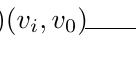
\begin{tikzpicture}

  \tkzDefPoint(0,0){cvert}
  \tkzDrawPoint(cvert) \tkzLabelPoint[above](cvert){$(v_i,)$}

  \draw[->] (1,0) -> (2,0);

  \tkzDefPoint(3,0){fvert}
  \tkzDrawPoint(fvert) \tkzLabelPoint[above](fvert){$(v_i,v_0)$}


\end{tikzpicture}

\vspace{2em}

% edge refinement
\begin{tikzpicture}

  \tkzDefPoint(0,0){cstart}
  \tkzDefPoint(3,0){cend}
  \tkzDrawSegment(cstart,cend)
  \tkzLabelSegment(cstart,cend){$(e_i,)$}

  \draw[->] (4,0) -> (5,0);

  \tkzDefPoint(6,0){fstart}
  \tkzDefPoint(11,0){fend}
  \tkzDefMidPoint(fstart,fend) \tkzGetPoint{fmid}

  \tkzDrawSegment(fstart,fmid) \tkzLabelSegment(fstart,fmid){$(e_i,e_0)$}
  \tkzDrawSegment(fmid,fend) \tkzLabelSegment(fmid,fend){$(e_i,e_1)$}
  \tkzDrawPoint(fmid) \tkzLabelPoint[below](fmid){$(e_i,v_0)$}

\end{tikzpicture}

\vspace{2em}

% cell refinement
\begin{tikzpicture}

  \tkzDefPoint(0,0){v0}
  \tkzDefShiftPoint[v0](60:5){v1}
  \tkzDefShiftPoint[v0](0:5){v2}
  \tkzDrawPolygon[style=dashed](v0,v1,v2)

  \tkzDefBarycentricPoint(v0=1,v1=1,v2=1) \tkzGetPoint{c0}
  \tkzLabelPoint[centered](c0){$c_i$}

  \draw[->] (5,{5/4*sqrt(3)}) -- (6,{5/4*sqrt(3)});

  \tkzDefPoint(7,0){fv0}
  \tkzDefShiftPoint[fv0](60:5){fv1}
  \tkzDefShiftPoint[fv0](0:5){fv2}
  \tkzDrawPolygon[style=dashed](fv0,fv1,fv2)

  \tkzDefMidPoint(fv0,fv1) \tkzGetPoint{fe0}
  \tkzDefMidPoint(fv1,fv2) \tkzGetPoint{fe1}
  \tkzDefMidPoint(fv2,fv0) \tkzGetPoint{fe2}

  \tkzDrawSegment(fe0,fe1)
  \tkzDrawSegment(fe1,fe2)
  \tkzDrawSegment(fe2,fe0)

  \tkzDefBarycentricPoint(fv0=1,fe0=1,fe2=1) \tkzGetPoint{fc0}
  \tkzLabelPoint[centered](fc0){$(c_i,c_0)$}

  \tkzDefBarycentricPoint(fe0=1,fe1=1,fe2=1) \tkzGetPoint{fc1}
  \tkzLabelPoint[centered](fc1){$(c_i,c_1)$}

  \tkzDefBarycentricPoint(fv1=1,fe0=1,fe1=1) \tkzGetPoint{fc2}
  \tkzLabelPoint[centered](fc2){$(c_i,c_2)$}

  \tkzDefBarycentricPoint(fv2=1,fe1=1,fe2=1) \tkzGetPoint{fc3}
  \tkzLabelPoint[centered](fc3){$(c_i,c_3)$}

  % edges (2/3 along)
  \tkzDefBarycentricPoint(fe2=1,fe0=2) \tkzGetPoint{e0labeldest}
  \tkzDefBarycentricPoint(fe0=1,fe1=2) \tkzGetPoint{e1labeldest}
  \tkzDefBarycentricPoint(fe1=2,fe2=1) \tkzGetPoint{e2labeldest}

  \node [xshift=-1.6cm,yshift=.2cm] (e0labelsrc) at (e0labeldest) {$(c_i,e_0)$};
  \draw (e0labelsrc) -- (e0labeldest);

  \node [xshift=1.2cm,yshift=.9cm] (e1labelsrc) at (e1labeldest) {$(c_i,e_1)$};
  \draw (e1labelsrc) -- (e1labeldest);

  \node [xshift=1.5cm,yshift=.4cm] (e2labelsrc) at (e2labeldest) {$(c_i,e_2)$};
  \draw (e2labelsrc) -- (e2labeldest);



\end{tikzpicture}

\subsection{Data layout transformations}

% mixed reordering
\begin{tikzpicture}[y=-1cm]
  \begin{scope}[xshift=3.5cm, yshift=0cm]
    \filldraw[draw=black, fill=white] (0,0) rectangle (1,1);
    \filldraw[draw=black, fill=white] (1,0) rectangle (2,1);
    \node[at={(.5,.5)}, ptlabel] {$V_0$};
    \node[at={(1.5,.5)}, ptlabel] {$V_1$};
  \end{scope}

  \begin{scope}[yshift=-2cm]
    \begin{scope}[xshift=0cm]
      \fill[lightgray] (0,0) rectangle (4,1);
      \filldraw[draw=black, fill=white] (0.5,0) rectangle (1.5,1);
      \filldraw[draw=black, fill=white] (1.5,0) rectangle (2.5,1);
      \filldraw[draw=black, fill=white] (2.5,0) rectangle (3.5,1);
      \node[at={(1,.5)}, ptlabel] {$c_0$};
      \node[at={(2,.5)}, ptlabel] {$v_1$};
      \node[at={(3,.5)}, ptlabel] {$c_4$};
      \draw (0,0) -- (4,0);
      \draw (0,1) -- (4,1);
    \end{scope}

    \begin{scope}[xshift=5cm]
      \fill[lightgray] (0,0) rectangle (4,1);
      \filldraw[draw=black, fill=white] (0.5,0) rectangle (1.5,1);
      \filldraw[draw=black, fill=white] (1.5,0) rectangle (2.5,1);
      \filldraw[draw=black, fill=white] (2.5,0) rectangle (3.5,1);
      \node[at={(1,.5)}, ptlabel] {$c_0$};
      \node[at={(2,.5)}, ptlabel] {$v_1$};
      \node[at={(3,.5)}, ptlabel] {$c_4$};
      \draw (0,0) -- (4,0);
      \draw (0,1) -- (4,1);
    \end{scope}
  \end{scope}

  \draw (3.5,1) -- (0,2);
  \draw (4.5,1) -- (4,2);
  \draw (4.5,1) -- ({0+5},2);
  \draw (5.5,1) -- ({4+5},2);

\end{tikzpicture}

% one could introduce a proper tensor language to express things (like Simit) - currently only
% focussed on the packing part
